%===============================================================================
% LaTeX sjabloon voor de bachelorproef toegepaste informatica aan HOGENT
% Meer info op https://github.com/HoGentTIN/latex-hogent-report
%===============================================================================

\documentclass[dutch,dit,thesis]{hogentreport}

% TODO:
% - If necessary, replace the option `dit`' with your own department!
%   Valid entries are dbo, dbt, dgz, dit, dlo, dog, dsa, soa
% - If you write your thesis in English (remark: only possible after getting
%   explicit approval!), remove the option "dutch," or replace with "english".

\usepackage{lipsum} % For blind text, can be removed after adding actual content

%% Pictures to include in the text can be put in the graphics/ folder
\graphicspath{{../graphics/}}

%% For source code highlighting, requires pygments to be installed
%% Compile with the -shell-escape flag!
%% \usepackage[chapter]{minted}
%% If you compile with the make_thesis.{bat,sh} script, use the following
%% import instead:
\usepackage[chapter,outputdir=../output]{minted}
\usemintedstyle{solarized-light}

%% Formatting for minted environments.
\setminted{%
    autogobble,
    frame=lines,
    breaklines,
    linenos,
    tabsize=4
}

%% Ensure the list of listings is in the table of contents
\renewcommand\listoflistingscaption{%
    \IfLanguageName{dutch}{Lijst van codefragmenten}{List of listings}
}
\renewcommand\listingscaption{%
    \IfLanguageName{dutch}{Codefragment}{Listing}
}
\renewcommand*\listoflistings{%
    \cleardoublepage\phantomsection\addcontentsline{toc}{chapter}{\listoflistingscaption}%
    \listof{listing}{\listoflistingscaption}%
}

% Other packages not already included can be imported here

%%---------- Document metadata -------------------------------------------------
% TODO: Replace this with your own information
\author{Ernst Aarden}
\supervisor{Dhr. F. Van Houte}
\cosupervisor{Mevr. S. Beeckman}
\title[Optionele ondertitel]%
    {Titel van de bachelorproef}
\academicyear{\advance\year by -1 \the\year--\advance\year by 1 \the\year}
\examperiod{1}
\degreesought{\IfLanguageName{dutch}{Professionele bachelor in de toegepaste informatica}{Bachelor of applied computer science}}
\partialthesis{false} %% To display 'in partial fulfilment'
%\institution{Internshipcompany BVBA.}

%% Add global exceptions to the hyphenation here
\hyphenation{back-slash}

%% The bibliography (style and settings are  found in hogentthesis.cls)
\addbibresource{bachproef.bib}            %% Bibliography file
\addbibresource{../voorstel/voorstel.bib} %% Bibliography research proposal
\defbibheading{bibempty}{}

%% Prevent empty pages for right-handed chapter starts in twoside mode
\renewcommand{\cleardoublepage}{\clearpage}

\renewcommand{\arraystretch}{1.2}

%% Content starts here.
\begin{document}

%---------- Front matter -------------------------------------------------------

\frontmatter

\hypersetup{pageanchor=false} %% Disable page numbering references
%% Render a Dutch outer title page if the main language is English
\IfLanguageName{english}{%
    %% If necessary, information can be changed here
    \degreesought{Professionele Bachelor toegepaste informatica}%
    \begin{otherlanguage}{dutch}%
       \maketitle%
    \end{otherlanguage}%
}{}

%% Generates title page content
\maketitle
\hypersetup{pageanchor=true}

%%=============================================================================
%% Voorwoord
%%=============================================================================

\chapter*{\IfLanguageName{dutch}{Woord vooraf}{Preface}}%
\label{ch:voorwoord}

%% Het voorwoord is het enige deel van de bachelorproef waar je vanuit je
%% eigen standpunt (``ik-vorm'') mag schrijven. Je kan hier bv. motiveren
%% waarom jij het onderwerp wil bespreken.
%% Vergeet ook niet te bedanken wie je geholpen/gesteund/... heeft
Als fanclubfotograaf en trouwe supporter van Lindemans Aalst is deze club al jarenlang een vaste waarde in mijn leven. Het spreekt dan ook voor zich dat ik met veel enthousiasme mijn bachelorproef wou wijden aan een onderwerp dat me nauw aan het hart ligt.

Voor de totstandkoming van deze bachelorproef heb ik dan ook op de steun van verschillende mensen mogen rekenen, aan wie ik graag mijn oprechte dank wil uitspreken. In het bijzonder wil ik mijn co-promotor, Dhr. Joost Van Kerckhove, bedanken voor zijn bereidwillige medewerking en de gedeelde expertise. Eveneens een welgemeende dank aan de staf van Lindemans Aalst voor het aanleveren van de nodige statistieken, gegevens en achtergrondinformatie die deze bachelorproef mee vorm hebben gegeven.

Daarnaast wil ik mevrouw Lotte Van Steenberghe bedanken voor haar begeleiding en ondersteuning tijdens het hele traject.

Ook een bijzonder woord van dank aan mijn ouders en zus. Hun onvoorwaardelijke steun, eindeloze aanmoediging en begripvolle luisterend oor zijn voor mij van onschatbare waarde geweest in deze periode. Ze hebben me de rust, motivatie en ruimte gegeven om dit project tot een goed einde te brengen.

Tot slot wil ik ook mijn vriend Lennert bedanken, die steeds klaarstond om mijn vele vragen over de statistieken te beantwoorden.

Aan iedereen die op een of andere manier heeft bijgedragen: dankjewel. Zonder jullie hulp was dit werk niet geworden wat het nu is.

\vspace{5mm} %5mm vertical space

Ik wens u veel leesplezier toe!

Youna Noynaert
%%=============================================================================
%% Samenvatting
%%=============================================================================

% De "abstract" of samenvatting is een kernachtige (~ 1 blz. voor een
% thesis) synthese van het document.
%
% Een goede abstract biedt een kernachtig antwoord op volgende vragen:
%
% 1. Waarover gaat de bachelorproef?
% 2. Waarom heb je er over geschreven?
% 3. Hoe heb je het onderzoek uitgevoerd?
% 4. Wat waren de resultaten? Wat blijkt uit je onderzoek?
% 5. Wat betekenen je resultaten? Wat is de relevantie voor het werkveld?
%
% Daarom bestaat een abstract uit volgende componenten:
%
% - inleiding + kaderen thema
% - probleemstelling
% - (centrale) onderzoeksvraag
% - onderzoeksdoelstelling
% - methodologie
% - resultaten (beperk tot de belangrijkste, relevant voor de onderzoeksvraag)
% - conclusies, aanbevelingen, beperkingen
%
% LET OP! Een samenvatting is GEEN voorwoord!

%%---------- Nederlandse samenvatting -----------------------------------------
%
% Als je je bachelorproef in het Engels schrijft, moet je eerst een
% Nederlandse samenvatting invoegen. Haal daarvoor onderstaande code uit
% commentaar.
% Wie zijn bachelorproef in het Nederlands schrijft, kan dit negeren, de inhoud
% wordt niet in het document ingevoegd.

\IfLanguageName{english}{%
\selectlanguage{dutch}
\chapter*{Samenvatting}
\lipsum[1-4]
\selectlanguage{english}
}{}

%%---------- Samenvatting -----------------------------------------------------
% De samenvatting in de hoofdtaal van het document

\chapter*{\IfLanguageName{dutch}{Samenvatting}{Abstract}}
In de sportwereld, en specifiek in volleybal, spelen wedstrijd- en spelerstatistieken een cruciale rol bij prestatieverbetering en strategische besluitvorming. Bij volleybalclub Lindemans Aalst worden wedstrijdstatistieken momenteel handmatig bijgehouden, terwijl er tijdens trainingen zelfs geen gegevens worden vastgelegd. Dit onderzoek richt zich op de mogelijkheden en voordelen van het automatiseren van deze statistieken met behulp van AI-technologie, om zo een competitief voordeel te behalen.

De centrale onderzoeksvraag luidt: \textit{Welke bestaande AI-oplossing voor het automatiseren van volleybalstatistieken biedt de meeste voordelen voor Lindemans Aalst, zowel tijdens wedstrijden als trainingen?} Het doel is om via een vergelijkende studie de meest geschikte AI-technologie te selecteren en implementeren, rekening houdend met nauwkeurigheid, gebruiksgemak, kosten en toepasbaarheid binnen de clubcontext.

De methodologie bestaat uit een literatuurstudie naar bestaande AI-oplossingen voor sportanalyse, interviews met stakeholders binnen de club om functionele en technische vereisten in kaart te brengen, en een vergelijkende studie van AI-systemen. De best presterende oplossing wordt getest in een proof-of-concept binnen de dagelijkse werking van Lindemans Aalst.

Uit het onderzoek wordt verwacht dat AI-gestuurde statistiekenregistratie de nauwkeurigheid en snelheid van data-analyse aanzienlijk zal verbeteren. Hierdoor kunnen coaches beter onderbouwde strategische beslissingen nemen en de spelersontwikkeling optimaliseren. Daarnaast blijkt uit de analyse dat geen enkele andere club in Liga A momenteel AI-technologie gebruikt voor het verzamelen en analyseren van statistieken. Dit biedt Lindemans Aalst de kans om een pioniersrol te vervullen en een aanzienlijk competitief voordeel te behalen.

Naast directe voordelen voor Lindemans Aalst, kunnen de bevindingen ook waardevol zijn voor andere sportclubs die AI-technologie willen integreren in hun trainings- en wedstrijdanalyse.


%---------- Inhoud, lijst figuren, ... -----------------------------------------

\tableofcontents

% In a list of figures, the complete caption will be included. To prevent this,
% ALWAYS add a short description in the caption!
%
%  \caption[short description]{elaborate description}
%
% If you do, only the short description will be used in the list of figures

\listoffigures

% If you included tables and/or source code listings, uncomment the appropriate
% lines.
\listoftables

\listoflistings

% Als je een lijst van afkortingen of termen wil toevoegen, dan hoort die
% hier thuis. Gebruik bijvoorbeeld de ``glossaries'' package.
% https://www.overleaf.com/learn/latex/Glossaries

%---------- Kern ---------------------------------------------------------------

\mainmatter{}

% De eerste hoofdstukken van een bachelorproef zijn meestal een inleiding op
% het onderwerp, literatuurstudie en verantwoording methodologie.
% Aarzel niet om een meer beschrijvende titel aan deze hoofdstukken te geven of
% om bijvoorbeeld de inleiding en/of stand van zaken over meerdere hoofdstukken
% te verspreiden!

%%=============================================================================
%% Inleiding
%%=============================================================================

\chapter{\IfLanguageName{dutch}{Inleiding}{Introduction}}%
\label{ch:inleiding}

Datagedreven besluitvorming wordt steeds belangrijker in de sportwereld. Professionele sportteams maken gebruik van geavanceerde analysetools om prestaties te meten, tactieken te optimaliseren en spelersontwikkeling te bevorderen. In de volleybalwereld worden statistieken al decennialang gebruikt om inzicht te krijgen in spelpatronen en individuele prestaties. Traditioneel worden deze gegevens echter handmatig verzameld en geanalyseerd, wat tijdrovend is en ruimte laat voor menselijke fouten.

\section{\IfLanguageName{dutch}{Probleemstelling}{Problem Statement}}%
\label{sec:probleemstelling}

Hoewel veel sporten de transitie naar geautomatiseerde data-analyse al hebben gemaakt, gebeurt dit in het Belgische volleybal nog nauwelijks. Geen enkele club in Liga A maakt momenteel gebruik van AI-technologie om statistieken te verzamelen en analyseren. Hierdoor blijft een waardevolle bron van informatie grotendeels onbenut. Het ontbreken van geautomatiseerde statistieken zorgt ervoor dat beslissingen vaak gebaseerd worden op subjectieve observaties in plaats van op objectieve data. Dit kan leiden tot minder nauwkeurige analyses en gemiste optimalisatiemogelijkheden.

\section{\IfLanguageName{dutch}{Onderzoeksvraag}{Research question}}%
\label{sec:onderzoeksvraag}

Deze studie tracht een bestaande AI-oplossing te identificeren die de meeste voordelen biedt voor volleybalclub Lindemans Aalst, zowel tijdens wedstrijden als trainingen. De centrale onderzoeksvraag luidt als volgt: \textit{Welke bestaande AI-oplossing voor volleybalstatistieken biedt de meeste voordelen voor Lindemans Aalst, zowel tijdens wedstrijden als trainingen?}

Hiervoor werden de volgende vragen ook onderzocht:
\begin{itemize}
    \item Waarom zijn statistieken belangrijk in de sportwereld en specifiek in volleybal?
    \item Welke technologieën worden momenteel gebruikt voor het automatiseren van sportstatistieken?
    \item Hoe presteren bestaande AI-systemen voor het verzamelen en analyseren van volleybalstatistieken?
\end{itemize}

\section{\IfLanguageName{dutch}{Onderzoeksdoelstelling}{Research objective}}%
\label{sec:onderzoeksdoelstelling}

Het uiteindelijke doel is om te bepalen welke bestaande AI-oplossing het meest geschikt is voor de automatisering van volleybalstatistieken bij Lindemans Aalst. Dit gebeurt aan de hand van een vergelijkende studie van bestaande technologieën en een proof-of-concept binnen de clubcontext.

Het onderzoek richt zich op het identificeren van een oplossing die voldoet aan de volgende succescriteria:
\begin{itemize}
  \item \textbf{Nauwkeurigheid}: De AI-technologie moet minstens even accuraat zijn als handmatige registratie en idealiter een verbeterde databetrouwbaarheid bieden.
  \item \textbf{Snelheid}: De verwerkingstijd van statistieken moet aanzienlijk korter zijn dan bij manuele methoden, zodat coaches tijdens wedstrijden en trainingen in realtime bruikbare inzichten krijgen.
  \item \textbf{Gebruikersvriendelijkheid}: De technologie moet eenvoudig te gebruiken zijn voor coaches en data-analisten, zonder uitgebreide technische kennis.
  \item \textbf{Kostenefficiëntie}: De implementatie en het onderhoud van de technologie moeten financieel haalbaar zijn binnen de middelen van de club.
  \item \textbf{Toepasbaarheid}: De technologie moet compatibel zijn met de infrastructuur en werkwijze van Lindemans Aalst en gemakkelijk te integreren in hun dagelijkse werking.
\end{itemize}

Het beoogde eindresultaat van dit onderzoek is een verslag met aanbevelingen over de meest geschikte AI-oplossing, inclusief een analyse van de voor- en nadelen van de onderzochte systemen. Daarnaast wordt een proof-of-concept van de gekozen technologie uitgevoerd, waarbij het systeem wordt getest in een reële trainings- en wedstrijdomgeving. Op basis van deze praktijktest wordt een evaluatie gemaakt van de effectiviteit en de haalbaarheid van de implementatie op lange termijn.

Naast de directe voordelen voor Lindemans Aalst kan dit onderzoek ook als referentie dienen voor andere volleybalclubs in Liga A die overwegen om AI-technologie te integreren in hun statistiekenregistratie en wedstrijdanalyse.

\section{\IfLanguageName{dutch}{Opzet van deze bachelorproef}{Structure of this bachelor thesis}}%
\label{sec:opzet-bachelorproef}

% Het is gebruikelijk aan het einde van de inleiding een overzicht te
% geven van de opbouw van de rest van de tekst. Deze sectie bevat al een aanzet
% die je kan aanvullen/aanpassen in functie van je eigen tekst.

De rest van deze bachelorproef is als volgt opgebouwd:

In Hoofdstuk~\ref{ch:stand-van-zaken} wordt een overzicht gegeven van de stand van zaken binnen het onderzoeksdomein, op basis van een literatuurstudie.

In Hoofdstuk~\ref{ch:methodologie} wordt de methodologie toegelicht en worden de gebruikte onderzoekstechnieken besproken om een antwoord te kunnen formuleren op de onderzoeksvragen.

% Vul hier aan voor je eigen hoofstukken, één of twee zinnen per hoofdstuk
In Hoofdstuk~\ref{ch:requirementsanalyse} wordt de requirementsanalyse besproken, waarbij de functionele en technische eisen van de AI-oplossing in kaart worden gebracht.

In Hoofdstuk~\ref{ch:vergelijkendestudie} wordt een vergelijkende studie uitgevoerd van de geselecteerde AI-systemen, waarbij hun prestaties worden geëvalueerd op basis van nauwkeurigheid, snelheid en gebruiksgemak.	

In Hoofdstuk~\ref{ch:poc} wordt de proof-of-concept besproken, waarin het aanbevolen systeem wordt geïmplementeerd en getest binnen de dagelijkse werking van Lindemans Aalst.

In Hoofdstuk~\ref{ch:eindrapport} worden de resultaten van de proof-of-concept gepresenteerd en geanalyseerd. Dit hoofdstuk bevat ook een evaluatie van de effectiviteit en haalbaarheid van de implementatie op lange termijn.

In Hoofdstuk~\ref{ch:conclusie}, tenslotte, wordt de conclusie gegeven en een antwoord geformuleerd op de onderzoeksvragen. Daarbij wordt ook een aanzet gegeven voor toekomstig onderzoek binnen dit domein.
\chapter{\IfLanguageName{dutch}{Stand van zaken}{State of the art}}%
\label{ch:stand-van-zaken}

% Tip: Begin elk hoofdstuk met een paragraaf inleiding die beschrijft hoe
% dit hoofdstuk past binnen het geheel van de bachelorproef. Geef in het
% bijzonder aan wat de link is met het vorige en volgende hoofdstuk.

% Pas na deze inleidende paragraaf komt de eerste sectiehoofding.

% Dit hoofdstuk bevat je literatuurstudie. De inhoud gaat verder op de inleiding, maar zal het onderwerp van de bachelorproef *diepgaand* uitspitten. De bedoeling is dat de lezer na lezing van dit hoofdstuk helemaal op de hoogte is van de huidige stand van zaken (state-of-the-art) in het onderzoeksdomein. Iemand die niet vertrouwd is met het onderwerp, weet nu voldoende om de rest van het verhaal te kunnen volgen, zonder dat die er nog andere informatie moet over opzoeken \autocite{Pollefliet2011}.

% Je verwijst bij elke bewering die je doet, vakterm die je introduceert, enz.\ naar je bronnen. In \LaTeX{} kan dat met het commando \texttt{$\backslash${textcite\{\}}} of \texttt{$\backslash${autocite\{\}}}. Als argument van het commando geef je de ``sleutel'' van een ``record'' in een bibliografische databank in het Bib\LaTeX{}-formaat (een tekstbestand). Als je expliciet naar de auteur verwijst in de zin (narratieve referentie), gebruik je \texttt{$\backslash${}textcite\{\}}. Soms is de auteursnaam niet expliciet een onderdeel van de zin, dan gebruik je \texttt{$\backslash${}autocite\{\}} (referentie tussen haakjes). Dit gebruik je bv.~bij een citaat, of om in het bijschrift van een overgenomen afbeelding, broncode, tabel, enz. te verwijzen naar de bron. In de volgende paragraaf een voorbeeld van elk.

% \textcite{Knuth1998} schreef een van de standaardwerken over sorteer- en zoekalgoritmen. Experten zijn het erover eens dat cloud computing een interessante opportuniteit vormen, zowel voor gebruikers als voor dienstverleners op vlak van informatietechnologie~\autocite{Creeger2009}.

% Let er ook op: het \texttt{cite}-commando voor de punt, dus binnen de zin. Je verwijst meteen naar een bron in de eerste zin die erop gebaseerd is, dus niet pas op het einde van een paragraaf.


% \begin{figure}
%   \centering
%   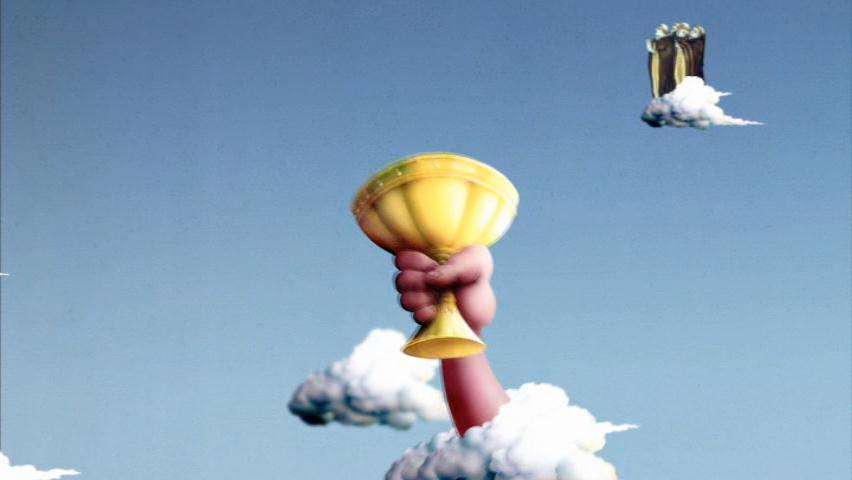
\includegraphics[width=0.8\textwidth]{grail.jpg}
%   \caption[Voorbeeld figuur.]{\label{fig:grail}Voorbeeld van invoegen van een figuur. Zorg altijd voor een uitgebreid bijschrift dat de figuur volledig beschrijft zonder in de tekst te moeten gaan zoeken. Vergeet ook je bronvermelding niet!}
% \end{figure}

% \begin{listing}
%   \begin{minted}{python}
%     import pandas as pd
%     import seaborn as sns

%     penguins = sns.load_dataset('penguins')
%     sns.relplot(data=penguins, x="flipper_length_mm", y="bill_length_mm", hue="species")
%   \end{minted}
%   \caption[Voorbeeld codefragment]{Voorbeeld van het invoegen van een codefragment.}
% \end{listing}

% \begin{table}
%   \centering
%   \begin{tabular}{lcr}
%     \toprule
%     \textbf{Kolom 1} & \textbf{Kolom 2} & \textbf{Kolom 3} \\
%     $\alpha$         & $\beta$          & $\gamma$         \\
%     \midrule
%     A                & 10.230           & a                \\
%     B                & 45.678           & b                \\
%     C                & 99.987           & c                \\
%     \bottomrule
%   \end{tabular}
%   \caption[Voorbeeld tabel]{\label{tab:example}Voorbeeld van een tabel.}
% \end{table}

Geautomatiseerde dataverzameling en -analyse spelen een steeds grotere rol in de professionele sportwereld, waar nauwkeurige statistieken noodzakelijk zijn voor prestatieverbetering en strategische besluitvorming. In de sport, in het bijzonder in volleybal, zorgt automatisering van statistiekenverzameling ervoor dat spelers en coaches beter inzicht krijgen in prestaties, waardoor training en wedstrijdvoorbereiding doelgerichter kunnen worden aangepakt.

\section{Belang van statistieken in de sportwereld}
Vooral technologieën zoals AI, computer vision en machine learning bieden nieuwe mogelijkheden om spelmomenten en spelersbewegingen nauwkeurig vast te leggen en te analyseren. De spelers- en matchstatistieken \autocite{Wahyuti2023} zijn van uiterst belang. Ze bieden niet alleen inzichten in de puntenregistratie van het team, maar ook in de tactische en technische aspecten van het spel. Volgens de studie is het belangrijk om een uitgebreid digitaal puntenregistratie bij te houden. Dit om fouten en verlies van gegevens, wat vaak voorkomt bij handmatige invoer, te minimaliseren. Uit onderzoek \autocite{Harabagiu2023} blijkt dat door gebruik van de statistische software Data Volley de efficiënte van een team met 6\% stijgt. De software identificeert de tekortkomingen en hierdoor kunnen individuele trainingsprogramma's opgesteld worden voor elke speler. Volgens \textcite{Ruiye2024} zijn de nauwkeurigheid en efficiëntie van de videoanalyse zeer belangrijk. Een innovatief videoanalysemodel gebaseerd op Bi-directional Long Short-Term Memory (BiLSTM) en aandachtsmechanismen behaalt een herkenningsnauwkeurigheid van meer dan 90\%.

Natuurlijk zijn er andere invloeden op de statistieken dan alleen de spelersprestaties \autocite{LopezSerrano2022}. Zo spelen volgens verschillende coaches het niveau van de tegenstander, het moment in een set, het scoreverschil, resultaat van de vorige set en het de competitieve druk een zeer grote in de analyse. Trainers pleiten ervoor dat er een geïntegreerde benadering is voor deze variabelen. Hierdoor wordt rekening gehouden met de specifieke omstandigheden van elke wedstrijd. Deze gegevens mogen niet geïsoleerd worden bekeken, maar juist in samenhang geanalyseerd. Bij verder onderzoek is het van essentieel belang dat coaches worden betrokken bij de ontwikkeling hiervan.

\section{Toepassing van kunstmatige intelligentie en data-analyse}
\textcite{Fadl2020} benadrukt het belang van moderne technologieën in de sport en hoe deze kunnen bijdragen aan het verbeteren van coachingsmethoden.

Om dit te bereiken, werd een beoordelingssysteem ontwikkeld waarmee coaches de bewegingsanalyse van spelers efficiënter kunnen uitvoeren. Dit systeem werd geëvalueerd door 200 ervaren volleybalcoaches en bleek binnen een korte tijdspanne van maximaal 15 minuten bruikbare inzichten te bieden. De methode omvatte verschillende analysecomponenten, zoals technische observatie, prestatiediagnose en trainingsinterventies, om coaches te helpen bij het plannen en optimaliseren van trainingssessies.
Uit de resultaten bleek dat AI-gestuurde bewegingsanalyse een effectief hulpmiddel is om trainers te ondersteunen bij het kwantificeren van prestaties en het identificeren van verbeterpunten.
Deze bevindingen onderstrepen hoe technologische vooruitgang kan bijdragen aan een betere trainingservaring, door coaches te voorzien van nauwkeurige en snelle analytische tools voor het verbeteren van de prestaties van hun spelers.

\textcite{Huang2023} ontwikkelen een AI-gestuurd model voor de detectie en herkenning van overtredingen in volleybal, ter vervanging van subjectieve scheidsrechtersoordelen. Het model maakt gebruik van videoverbeteringstechnologie en een combinatie van algoritmen, waaronder de wavelet-transformatie, de drie-frame verschilmethode en achtergrondsubtractie, om bewegende objecten te identificeren. De wavelet-transformatie is een techniek die signalen in verschillende frequenties analyseert en zowel tijd- als frequentiedomein-informatie biedt, wat helpt bij het extraheren van belangrijke kenmerken van bewegende objecten, zoals spelers en de bal. De drie-frame verschilmethode vergelijkt opeenvolgende frames in een video om veranderingen te detecteren, wat effectief helpt bij het identificeren van de beweging van objecten, zoals de bal en de spelers. Daarnaast wordt achtergrondsubtractie toegepast, waarbij het verschil tussen de huidige beeldinhoud en een vooraf gedefinieerd achtergrondmodel wordt berekend, zodat alleen de bewegende objecten ten opzichte van de achtergrond worden geïdentificeerd.
De verbeterde CamShift-trackingmethode, ondersteund door een Kalman-filter, optimaliseert de tracking van spelers door dynamisch de grootte en positie van zoekgebieden aan te passen op basis van de kleurverdeling van de objecten, wat zorgt voor nauwkeurige objectvolging. Bovendien wordt een Hidden Markov Model (HMM) ingezet voor de classificatie van overtredingen. Het HMM is een statistisch model dat de toestand van het spel op basis van sequentiële data analyseert en de waarschijnlijkheid van een overtreding voorspelt op basis van eerdere gedragingen en de huidige staat van het spel.
Uit experimentele resultaten blijkt dat het model een hoge herkenningsnauwkeurigheid heeft (99,76\%) en een gemiddelde foutmarge van 0,003. Hiermee biedt het een objectieve en betrouwbare methode voor scheidsrechtersbeslissingen, wat bijdraagt aan de eerlijkheid en nauwkeurigheid van arbitrage in volleybal. Dit onderzoek benadrukt de potentie van AI in sportanalyse en opent mogelijkheden voor bredere toepassingen in andere sporten.

\textcite{Liu2021} introduceren een innovatief model voor sportdata-visualisatie, het Video-based Effective Visualization Framework (VEVF). Dit model combineert kunstmatige intelligentie (AI) en big data-analyse om sportvideo's te classificeren en te analyseren, met als doel de prestaties van atleten te verbeteren en coaches en analisten van waardevolle inzichten te voorzien.
Het belang van data-visualisatie in de sportwereld wordt nogmaals benadrukt, vooral in het tijdperk van big data. Sportdata, zoals atleetprestaties, trainingsstatistieken en gezondheidsgegevens, kunnen worden gebruikt om betere spelstrategieën te ontwikkelen, blessures te verminderen en de prestaties van atleten te verbeteren. Het VEVF-model maakt gebruik van draagbare apparaten om real-time bewegingsdata van atleten te verzamelen en deze te visualiseren in een 3D-virtuele omgeving. Dit stelt coaches in staat om de prestaties van atleten beter te monitoren en toekomstige bewegingen te voorspellen.

\section{Gebruik van sensors en camera's voor dataverzameling}
Uit onderzoek van Xu \textcite{Sun2021} blijkt dat door de vooruitgang in elektronische en sensortechnologieën het mogelijk is geworden om menselijke bewegingen en spelmomenten nauwkeurig vast te leggen. In de sportwereld zijn sensoren en camera's steeds vaker te vinden op en naast het veld. Deze technologieën maken het mogelijk om realtime data te verzamelen over spelersposities, balbewegingen en spelsituaties door middel van sensoren aan de gewrichten van spelers te bevestigen. Door deze data te analyseren met behulp van AI-algoritmen kunnen coaches en analisten waardevolle inzichten verkrijgen in de prestaties en strategieën.

Het onderzoek van \textcite{Salim2024} richt zich op het optimaliseren van volleybaltraining door middle van geavanceerde sensortechnologie en data-analyse. Er wordt een innovatief platform gepresenteert dat gebruikmaakt van een drukgevoelige vloer en machine learning om zowel atleten als coaches te ondersteunen. Het systeem kan automatisch verschillende volleybalacties herkennen. Artificiële intelligentie gaat deze acties detecteren en direct feedback geven aan de spelers. Daarnaast kan het ook automatisch belangrijke speelmomenten markeren.
Naast analyse biedt het systeem ook interactieve leeromgevingen, waarbij trainingen dynamisch worden aangepast op basis van de waargenomen bewegingen van spelers. Dit wordt mogelijk gemaakt door een combinatie van machine learning-modellen, waaronder convolutionele neurale netwerken (CNN) en actieve datarepresentatie (ADR). Convolutionele neurale netwerken vormen een klasse van diepe neurale netwerken die bijzonder geschikt zijn voor de verwerking en analyse van visuele gegevens. Ze bootsen de werking van het menselijk visuele systeem na door gebruik te maken van convolutielagen, waarbij kleine filters of kernels over een afbeelding schuiven om patronen en kenmerken zoals randen, vormen en texturen te detecteren. Dit maakt CNN's zeer effectief voor taken zoals beeldherkenning, objectdetectie en actieclassificatie, wat cruciaal is in interactieve leeromgevingen waarbij spelersbewegingen worden geanalyseerd en gebruikt om trainingen dynamisch aan te passen. Deze technologieën behaalden een nauwkeurigheid tot 78,71\% bij het herkennen van acties.
Deze technologie heeft wel nog verdere verbeteringen nodig vooraleer het in de praktijk kan toegepast worden, maar het toont wel aan dat de manier waarop volleybaltrainingen vorm krijgen fundamenteel kunnen veranderen.

\textcite{Liang2023} concludeerden dat traditionele videoanalysemethode vaak te beperkt is voor de variabele omstandigheden zoals verlichting en achtergrond tijdens het spel. Skeletdata biedt hier een oplossing voor door de bewegingen van spelers te vereenvoudigen tot een netwerk van verbonden gewrichten. De complexiteit van de visuele gegevens vermindert hierdoor. De methode zou nog een extra assistentie kunnen bieden aan de coaches en spelers.

\section{Gebruik van machine learning voor analyse van volleybaldata}
De integratie van machine learning en digitale informatietechnologie in volleybal biedt nieuwe mogelijkheden voor prestatieverbetering en spelanalyse.

\textcite{Musa2021} onderzoeken welke factoren bijdragen aan het identificeren van getalenteerde volleybalspelers. Hierbij werd gekeken naar zowel fysieke kenmerken, zoals lengte, gewicht en leeftijd, als psychologische aspecten, waaronder mentale weerbaarheid en voorbereiding op wedstrijden. Door middel van machine learning werden spelers ingedeeld in twee prestatiecategorieën: hoogpresterend (HVP) en laagpresterend (LVP).
Uit de resultaten bleek dat gewicht, leeftijd en psychologische vaardigheden significante verschillen vertoonden tussen de twee groepen, terwijl lengte geen doorslaggevende factor was. Hoogpresterende spelers blonken vooral uit in mentale strategieën zoals zelfspraak, visualisatie en emotieregulatie, wat een belangrijke rol bleek te spelen bij succes op het veld.
Deze studie benadrukt het belang van zowel fysieke als mentale factoren bij het selecteren van talentvolle volleybalspelers. Daarnaast laat het zien hoe machine learning kan worden ingezet als hulpmiddel voor coaches bij het scouten en samenstellen van teams.

Het onderzoek van \textcite{Dai2021} richt zich op het gebruik van machine learning voor de analyse van volleybaldata. Het doel is om spelers en coaches meer inzicht te geven in de technische uitvoering van bewegingen, met name de smash zoals afgebeeld in figuur \ref{fig:spike} en de bijbehorende spieractiviteit. In het experiment werden twaalf volleybalspelers onderverdeeld in twee groepen: één groep gebruikte een preswing-techniek met beide armen (type A), terwijl de andere groep deze techniek niet toepaste (type B).
Door middel van kinematische, dynamische en elektromyografische analyses werden de verschillende fasen van de smash bestudeerd, van de aanloop en afzet tot het moment van raken. De resultaten toonden aan dat type A-spelers over het algemeen een betere balans hadden in spieractiviteit tussen beide zijden van het lichaam. Bij type B-spelers werd daarentegen een grotere afhankelijkheid van de beenspieren vastgesteld, wat suggereert dat zij compenseren voor het ontbreken van een preswing-beweging met de armen.
Daarnaast bleek dat de kracht die tijdens de sprong werd gegenereerd, bij type A hoger was dan bij type B, wat duidt op een efficiëntere energieoverdracht. Ook was er een verschil in de bijdrage van de rompspieren, waarbij de rechte buikspier bij type A een evenwichtige rol speelde, terwijl deze bij type B een dominante functie had.

\begin{figure}
  \centering
  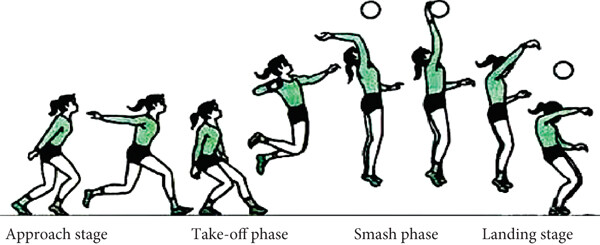
\includegraphics[width=0.8\textwidth]{spike.jpg}
  \caption{\label{fig:spike}Een reeks actiediagrammen van volleybal-spikes.}
  \autocite{Dai2021}
\end{figure}

Machine learning kan ook worden ingezet om blessures bij professionele volleyballers te monitoren en te voorspellen, volgens \textcite{Leeuw2021}. Door dagelijks gegevens te verzamelen over trainingsbelasting, sprongbelasting en welzijnsindicatoren, probeerden de onderzoekers inzicht te krijgen in het ontstaan en de ontwikkeling van overbelastingsblessures.
Voor dit onderzoek werden veertien topspelers gedurende 24 weken gevolgd. Ze vulden dagelijks vragenlijsten in over hun fysieke toestand en blessures, terwijl hun fysieke activiteiten en sprongbelasting werden geregistreerd via draagbare sensoren. De gegevens werden geanalyseerd met de machine learning-techniek Subgroup Discovery, waarmee verbanden tussen trainingsbelasting, welzijn en blessurerisico per individuele speler werden geïdentificeerd.
Uit de resultaten bleek dat verhoogde sprongbelasting een belangrijke voorspeller was van overbelastingsblessures, vooral aan de knieën. Daarnaast verschilden de risicofactoren per speler, wat het belang van een gepersonaliseerde aanpak onderstreept. Door patronen te herkennen in trainingsbelasting en blessureklachten, konden de onderzoekers gepersonaliseerd advies formuleren om blessures te helpen voorkomen.

\textcite{Yu2022} verkennen hoe kunstmatige neurale netwerken en genetische algoritmen kunnen bijdragen aan een betere beoordeling van serveer-, landings- en blokkeeracties. Door deze technologieën toe te passen, wordt niet alleen de reactietijd van spelers verbeterd, maar neemt ook de nauwkeurigheid van beslissingen toe, wat essentieel is voor training en blessurepreventie.
Verder worden clustering, regressieanalyse en informatieverwerking gebruikt om patronen in spelprestaties te identificeren en te voorspellen. De bevindingen tonen aan dat spelers met een hoger vaardigheidsniveau efficiënter tactische informatie verwerken en sneller reageren op speelsituaties. Dit onderzoek onderstreept de potentie van AI-gebaseerde technologieën in de sportwetenschap en biedt waardevolle inzichten voor coaching en prestatieanalyse.

\section{Bestaande AI-systemen voor sportstatistieken}
Er zijn verschillende AI-systemen beschikbaar die kunnen worden ingezet voor het verzamelen en analyseren van sportstatistieken. In tabel \ref{tab:tools} worden ze vergeleken met DataVolley, de tool die momenteel wordt gebruikt.

\begin{table}
  \centering
  \begin{tabular}{lcr}
    \toprule
    \textbf{Tool} & \textbf{Real-time} & \textbf{Video-input}\\
    \midrule
    DataVolley & Ja & Handmatige invoer \\
    Balltime AI & Nee & Opgenomen of live \\
    Volleymetrics & Nee & Opgenomen \\
    SportsVisio & Nee & Opgenomen of live \\
    SmashVision & Ja & Opgenomen of live \\
    \bottomrule
  \end{tabular}
  \caption[Korte vergelijking bestaande tools]{\label{tab:tools}Korte vergelijking bestaande tools}
\end{table}

Bij de analyse van volleybalwedstrijden en -trainingen worden verschillende tools ingezet om speldata te verzamelen en te verwerken. Deze tools verschillen op twee belangrijke aspecten: real-time verwerking en de wijze van video-input.

Sommige tools bieden real-time analyse, wat betekent dat gegevens direct tijdens de wedstrijd of training verwerkt en geanalyseerd worden. Dit is het geval bij Balltime AI en SportsVisio. Andere tools, zoals DataVolley en VolleyMetrics, bieden deze mogelijkheid niet en verwerken gegevens pas achteraf op basis van opgenomen videobeelden of handmatige invoer.

Naast real-time verwerking verschilt ook de manier waarop videobeelden worden gebruikt. DataVolley vereist een handmatige invoer van data met videobeelden, terwijl VolleyMetrics uitsluitend werkt met opgenomen video’s. De andere tools, zoals Balltime AI, Hudl Volleyball en SportsVisio, kunnen zowel opgenomen als live beelden verwerken. Dit maakt deze tools flexibeler in hun toepassing, omdat ze zowel achteraf als tijdens de wedstrijd analyses kunnen leveren.

De keuze voor een bepaalde analysetool hangt af van de specifieke behoeften van de gebruiker. Indien directe feedback gewenst is, zijn tools met real-time verwerking geschikter. Voor diepgaande analyse op basis van bestaande beelden kunnen niet-real-time tools een waardevolle aanvulling zijn.
%%=============================================================================
%% Methodologie
%%=============================================================================

\chapter{\IfLanguageName{dutch}{Methodologie}{Methodology}}%
\label{ch:methodologie}

%% In dit hoofstuk geef je een korte toelichting over hoe je te werk bent
%% gegaan. Verdeel je onderzoek in grote fasen, en licht in elke fase toe wat
%% de doelstelling was, welke deliverables daar uit gekomen zijn, en welke
%% onderzoeksmethoden je daarbij toegepast hebt. Verantwoord waarom je
%% op deze manier te werk gegaan bent.
%% 
%% Voorbeelden van zulke fasen zijn: literatuurstudie, opstellen van een
%% requirements-analyse, opstellen long-list (bij vergelijkende studie),
%% selectie van geschikte tools (bij vergelijkende studie, "short-list"),
%% opzetten testopstelling/PoC, uitvoeren testen en verzamelen
%% van resultaten, analyse van resultaten, ...
%%
%% !!!!! LET OP !!!!!
%%
%% Het is uitdrukkelijk NIET de bedoeling dat je het grootste deel van de corpus
%% van je bachelorproef in dit hoofstuk verwerkt! Dit hoofdstuk is eerder een
%% kort overzicht van je plan van aanpak.
%%
%% Maak voor elke fase (behalve het literatuuronderzoek) een NIEUW HOOFDSTUK aan
%% en geef het een gepaste titel.


\subsection{Fase 1: Literatuurstudie}
De literatuurstudie is bedoeld om inzicht te krijgen in de huidige stand van zaken met betrekking tot AI-systemen die geschikt zijn voor het verzamelen en analyseren van sportstatistieken. Ook wordt gekeken naar AI-modellen die in recent onderzoek effectief bleken voor sportanalyse. Daarnaast wordt ook de rol van sensors en camera's onderzocht. Waarom zijn statistieken belangrijk in de sportwereld en specifiek in volleybal? Deze vraag wordt beantwoord door het analyseren van academische publicaties en praktijkvoorbeelden. Daarnaast worden whitepapers en technische documentatie van bekende AI-tools, zoals Hudl, DataVolley, Second Spectrum en Balltime AI, bestudeerd.

De focus ligt hierbij op het beoordelen van nauwkeurigheid, snelheid, schaalbaarheid en kosten van deze systemen, omdat deze factoren belangrijk zijn voor de toepassing binnen Lindemans Aalst. Welke technologieën worden momenteel gebruikt voor het automatiseren van sportstatistieken? Dit wordt onderzocht door een overzicht te creëren van bestaande systemen en technologieën.

Aan het einde van deze fase wordt een overzichtsrapport opgesteld met de bevindingen, waarin ook een vergelijkingstabel wordt opgenomen die de sterke en zwakke punten van elk systeem schetst. Dit rapport vormt de basis voor de selectie van systemen die in latere fases verder onderzocht zullen worden.
\subsection{Fase 2: Interviews en requirementsanalyse}
In de tweede fase worden gestructureerde interviews afgenomen met de coaches, data-analisten en technische staf van Lindemans Aalst. Het doel van deze interviews is om een duidelijk beeld te krijgen van de functionele en technische eisen die de club stelt aan een geautomatiseerd statistieken systeem. Daarnaast wordt onderzocht in hoeverre de technische staf en spelers bereid zijn AI-technologie te omarmen en welke barrières er zijn bij implementatie. Ook wordt extra aandacht besteed aan de gebruiksvriendelijkheid van de systemen en de mate van benodigde technische kennis bij gebruikers. "Hoe presteren bestaande AI-systemen voor het verzamelen en analyseren van volleybalstatistieken?" en "Welke technologieën worden momenteel gebruikt voor het automatiseren van sportstatistieken?". Deze vragen worden besproken met stakeholders, waarbij hun ervaringen en verwachtingen worden genoteerd.

De requirementsanalyse richt zich op de statistieken die essentieel zijn voor de club en op specifieke analyses die coaches tijdens wedstrijden en trainingen nodig hebben. De inzichten uit deze gesprekken worden verwerkt in een requirementsdocument, dat de functionele en technische vereisten vastlegt. Dit document vormt een referentiepunt voor de vergelijkende analyse van de AI-systemen in de volgende fase.
\subsection{Fase 3: Vergelijkende studie van AI-systemen}
In deze fase worden de geselecteerde AI-systemen geëvalueerd op basis van nauwkeurigheid, snelheid en gebruiksgemak, om objectief te bepalen welke oplossing het best aansluit bij de eisen van Lindemans Aalst. Hiervoor wordt gebruikgemaakt van eerder verzamelde datasets van match- en trainingsgegevens. "Hoe presteren bestaande AI-systemen voor het verzamelen en analyseren van volleybalstatistieken?" wordt verder onderzocht door de prestaties van de systemen in de praktijk te testen en te vergelijken met handmatig geregistreerde data.

De systemen worden getest op hun vermogen om deze data nauwkeurig en snel te verwerken. Hierbij wordt niet alleen gekeken naar nauwkeurigheid en snelheid, maar ook naar de integratie met de bestaande infrastructuur van Lindemans Aalst. Daarnaast worden skeletgebaseerde AI-systemen zoals beschreven in de literatuurstudie meegenomen in de evaluatie, om hun potentieel binnen volleybalanalyse te beoordelen. De resultaten worden gepresenteerd in een rapport met grafieken en tabellen die de prestaties van elk systeem visueel weergeven. Het rapport bevat ook een concrete aanbeveling van het systeem dat het meest geschikt lijkt voor implementatie, op basis van de vergelijking.
\subsection{Fase 4: Proof of concept en praktijktest}
Na de vergelijkende studie wordt het aanbevolen systeem geïmplementeerd als proof of concept (PoC) bij Lindemans Aalst, op voorwaarde dat het seizoen nog bezig is. Deze praktijktest heeft als doel te valideren of het systeem daadwerkelijk voldoet aan de functionele en technische eisen van de club. Gedurende deze periode verzamelt het systeem automatisch gegevens tijdens trainingen en wedstrijden, zodat coaches en analisten het gebruiksgemak en de nauwkeurigheid van de automatisering kunnen evalueren. De prestaties van AI worden vergeleken met de traditionele methode om te bepalen of AI een significante meerwaarde biedt."

De prestaties van het PoC-systeem worden vergeleken met handmatig geregistreerde gegevens en de feedback van de coaches over de gebruiksvriendelijkheid wordt verzameld. Aan het einde van deze fase wordt een validatierapport opgesteld, waarin de kwantitatieve resultaten van het geautomatiseerde systeem zijn opgenomen, evenals eventuele aanbevelingen voor optimalisatie.
\subsection{Fase 5: Analyse en eindrapport}
In de laatste fase worden de resultaten van het onderzoek geanalyseerd en samengebracht in een eindrapport. Dit rapport bevat een grondige analyse van de prestaties van het PoC-systeem en conclusies over de mate waarin het systeem de doelstellingen van Lindemans Aalst ondersteunt. "Waarom zijn statistieken belangrijk in de sportwereld en specifiek in volleybal?" wordt in deze fase opnieuw geëvalueerd op basis van de praktische resultaten.

De data uit de eerdere fases worden statistisch geanalyseerd om objectieve conclusies te trekken over de invloed van automatisering op de nauwkeurigheid en snelheid van statistiekenregistratie. Het rapport bevat zowel aanbevelingen voor de club over de definitieve implementatie van het AI-systeem als suggesties voor toekomstige optimalisaties.


% Voeg hier je eigen hoofdstukken toe die de ``corpus'' van je bachelorproef
% vormen. De structuur en titels hangen af van je eigen onderzoek. Je kan bv.
% elke fase in je onderzoek in een apart hoofdstuk bespreken.

%\input{...}
%\input{...}
%...

%%=============================================================================
%% Conclusie
%%=============================================================================

\chapter{Conclusie}%
\label{ch:conclusie}

% Trek een duidelijke conclusie, in de vorm van een antwoord op de
% onderzoeksvra(a)g(en). Wat was jouw bijdrage aan het onderzoeksdomein en
% hoe biedt dit meerwaarde aan het vakgebied/doelgroep? 
% Reflecteer kritisch over het resultaat. In Engelse teksten wordt deze sectie
% ``Discussion'' genoemd. Had je deze uitkomst verwacht? Zijn er zaken die nog
% niet duidelijk zijn?
% Heeft het onderzoek geleid tot nieuwe vragen die uitnodigen tot verder 
%onderzoek?

Deze bachelorproef onderzocht welke bestaande AI-oplossing voor het automatiseren van volleybalstatistieken het meest geschikt is voor volleybalclub Lindemans Aalst. De aanleiding hiervoor was het ontbreken van geautomatiseerde dataverzameling binnen de club, wat de nauwkeurigheid, snelheid en bruikbaarheid van statistieken beperkte tijdens zowel trainingen als wedstrijden.

Uit de literatuurstudie bleek duidelijk dat AI en machine learning-technologieën al succesvol worden toegepast in verschillende sportdisciplines en aanzienlijke meerwaarde bieden in termen van prestatieanalyse, trainingsoptimalisatie en blessurepreventie. Er werd ook vastgesteld dat in de Liga A van het Belgische volleybal geen enkele club op dit moment gebruikmaakt van AI voor statistiekenverzameling, wat een strategisch voordeel biedt voor Lindemans Aalst om als pionier op te treden.

De requirementsanalyse, gevoed door interviews met coaches, scouters en stafleden, bracht de functionele en technische noden van de club in kaart. Hieruit bleek onder meer de nood aan real-time feedback, een hoge nauwkeurigheid van dataregistratie, gebruiksvriendelijkheid en integratiemogelijkheden met bestaande systemen zoals DataVolley. Daarnaast werd de wens uitgesproken om repetitieve taken te automatiseren en subjectieve fouten bij manuele invoer te minimaliseren.

De vergelijkende studie van bestaande AI-systemen identificeerde Balltime AI als het meest geschikte systeem voor de clubcontext, op basis van criteria zoals nauwkeurigheid, real-time verwerking, compatibiliteit, outputformaten en kosten. Dit systeem werd vervolgens getest in een proof-of-concept tijdens officiële wedstrijden.

Uit de analyse van de praktijktesten bleek dat Balltime AI in staat was om de meeste statistieken even accuraat en in sommige gevallen zelfs accurater dan de manuele methode te registreren. De verwerking gebeurde bovendien sneller en leverde realtime inzichten op die tijdens de wedstrijd benut konden worden. De feedback van de coaches bevestigde de gebruiksvriendelijkheid van het systeem en onderstreepte de meerwaarde van de automatische dataverwerking voor strategische besluitvorming.

Op basis van de resultaten van het onderzoek kan geconcludeerd worden dat automatisering van statistieken via AI een duidelijke meerwaarde biedt voor Lindemans Aalst. Niet alleen worden statistieken sneller en betrouwbaarder verzameld, maar het stelt de technische staf ook in staat om sneller te anticiperen op spelontwikkelingen. De club kan hiermee een voortrekkersrol opnemen binnen de Belgische volleybalwereld.

Tot slot biedt dit onderzoek ook aanbevelingen voor de verdere implementatie van AI binnen sportcontexten, met aandacht voor trainingsmogelijkheden, technische ondersteuning en integratie met bestaande software-infrastructuren. Verder onderzoek kan zich richten op het uitbreiden van AI-analyse naar individuele spelersontwikkeling en blessurepreventie, alsook de toepassing van AI in andere sportdisciplines.


%---------- Bijlagen -----------------------------------------------------------

\appendix

\chapter{Onderzoeksvoorstel}

Het onderwerp van deze bachelorproef is gebaseerd op een onderzoeksvoorstel dat vooraf werd beoordeeld door de promotor. Dat voorstel is opgenomen in deze bijlage.

%% TODO: 
%\section*{Samenvatting}

% Kopieer en plak hier de samenvatting (abstract) van je onderzoeksvoorstel.

% Verwijzing naar het bestand met de inhoud van het onderzoeksvoorstel
%---------- Inleiding ---------------------------------------------------------

\section{Inleiding}%
\label{sec:inleiding}

Match- en spelerstatistieken zijn van essentieel belang in de sportwereld. Waarom zijn statistieken belangrijk in de sportwereld en specifiek in volleybal? Bij Lindemans Aalst is het verzamelen van deze gegevens echter nog zeer tijdrovend. Tijdens wedstrijden worden statistieken handmatig bijgehouden, terwijl er tijdens trainingen zelfs geen gegevens worden verzameld. Dit handmatige proces is niet alleen inefficiënt, maar kan ook leiden tot inconsistenties in de data.

Automatisering van statistieken biedt potentieel voor een systeem dat in staat is realtime statistieken vast te leggen, zowel tijdens wedstrijden als trainingen, wat leidt tot een efficiënte en betrouwbare dataverzameling. Welke technologieën worden momenteel gebruikt voor het automatiseren van sportstatistieken? Hoe presteren bestaande AI-systemen voor het verzamelen en analyseren van volleybalstatistieken?

Automatisering zou ervoor zorgen dat er minder fouten aanwezig zijn en dat de statistieken sneller beschikbaar zijn. Dit zou er dan weer voor zorgen dat de coaches sneller en beter beslissingen kunnen maken. Daarom dus: \textit{"Welke bestaande AI-oplossing voor het automatiseren van volleybalstatistieken biedt de meeste voordelen voor Lindemans Aalst, zowel tijdens wedstrijden als trainingen?"}
%---------- Stand van zaken ---------------------------------------------------

\section{Literatuurstudie}%
\label{sec:literatuurstudie}
% Voor literatuurverwijzingen zijn er twee belangrijke commando's:
% \autocite{KEY} => (Auteur, jaartal) Gebruik dit als de naam van de auteur
%   geen onderdeel is van de zin.
% \textcite{KEY} => Auteur (jaartal)  Gebruik dit als de auteursnaam wel een
%   functie heeft in de zin (bv. ``Uit onderzoek door Doll & Hill (1954) bleek
%   ...'')
% Inleiding, wat is het belang van statistieken in de sportwereld
Geautomatiseerde dataverzameling en -analyse spelen een steeds grotere rol in de professionele sportwereld, waar nauwkeurige statistieken noodzakelijk zijn voor prestatieverbetering en strategische besluitvorming. In de sport, in het bijzonder in volleybal, zorgt automatisering van statistiekenverzameling ervoor dat spelers en coaches beter inzicht krijgen in prestaties, waardoor training en wedstrijdvoorbereiding doelgerichter kunnen worden aangepakt.
\subsection{Belang van statistieken in de sportwereld}
Vooral technologieën zoals AI, computer vision en machine learning bieden nieuwe mogelijkheden om spelmomenten en spelersbewegingen nauwkeurig vast te leggen en te analyseren. De spelers- en matchstatistieken \autocite{Wahyuti2023} zijn van uiterst belang. Ze bieden niet alleen inzichten in de puntenregistratie van het team, maar ook in de tactische en technische aspecten van het spel. Volgens de studie is het belangrijk om een uitgebreid digitaal puntenregistratie bij te houden. Dit om fouten en verlies van gegevens te minimaliseren. Dit komt echter vaak voor bij handmatige invoer. Uit onderzoek \autocite{Harabagiu2023} blijkt dat door het gebruik van door gebruik van de statistische software Data Volley de efficiënte van een team met 6\% stijgt. De software identificeert de tekortkomingen en hierdoor kunnen individuele trainingsprogramma's opgesteld worden voor elke speler. Volgens \textcite{Ruiye2024} zijn de nauwkeurigheid en efficiëntie van de videoanalyse zeer belangrijk. Een innovatief videoanalysemodel gebaseerd op Bi-directional Long Short-Term Memory (BiLSTM) en aandachtsmechanismen behaalt een herkenningsnauwkeurigheid van meer dan 90\%.

Natuurlijk zijn er andere invloeden op de statistieken dan alleen de spelersprestaties \autocite{LopezSerrano2022}. Zo spelen volgens verschillende coaches het niveau van de tegenstander, het moment in een set, het scoreverschil, resultaat van de vorige set en het de competitieve druk een zeer grote in de analyse. Trainers pleiten ervoor dat er een geïntegreerde benadering is voor deze variabelen. Hierdoor wordt rekening gehouden met de specifieke omstandigheden van elke wedstrijd. Deze gegevens mogen niet geïsoleerd worden bekeken, maar juist in samenhang geanalyseerd. Bij verder onderzoek is het van essentieel belang dat coaches worden betrokken bij de ontwikkeling hiervan.
% Bestaande AI-oplossingen voor sportstatistieken

% Gebruik van sensors en camera's voor dataverzameling
\subsection{Gebruik van sensors en camera's voor dataverzameling}
Uit onderzoek van Xu \textcite{Sun2021} blijkt dat door de vooruitgang in elektronische en sensortechnologieën is het mogelijk geworden om menselijke bewegingen en spelmomenten nauwkeurig vast te leggen. In de sportwereld zijn sensoren en camera's steeds vaker te vinden op en naast het veld. Deze technologieën maken het mogelijk om realtime data te verzamelen over spelersposities, balbewegingen en spelsituaties door middel van sensoren aan de gewrichten van spelers te bevestigen. Door deze data te analyseren met behulp van AI-algoritmen kunnen coaches en analisten waardevolle inzichten verkrijgen in de prestaties en strategieën.

\textcite{Liang2023} concludeerden dat traditionele videoanalysemethode vaak te beperkt zijn voor de variabele omstandigheden zoals verlichting en achtergrond tijdens het spel. Skeletdata biedt hier een oplossing voor door de bewegingen van spelers te vereenvoudigen tot een netwerk van verbonden gewrichten. De complexiteit van de visuele gegevens vermindert hierdoor. De methode zou nog een extra assistentie kunnen bieden aan de coaches en spelers.
%---------- Methodologie ------------------------------------------------------
\section{Methodologie}%
\label{sec:methodologie}

Elke week die beschreven wordt bestaat uit 1 volledige dag werk aan de bachelorproef.
\subsection{Fase 1: Literatuurstudie}
De literatuurstudie is bedoeld om inzicht te krijgen in de huidige stand van zaken met betrekking tot AI-systemen die geschikt zijn voor het verzamelen en analyseren van sportstatistieken. Waarom zijn statistieken belangrijk in de sportwereld en specifiek in volleybal? Deze vraag wordt beantwoord door het analyseren van academische publicaties en praktijkvoorbeelden. Daarnaast worden whitepapers en technische documentatie van bekende AI-tools, zoals Hudl, DataVolley, Second Spectrum en Balltime AI, bestudeerd.

De focus ligt hierbij op het beoordelen van nauwkeurigheid, snelheid, schaalbaarheid en kosten van deze systemen, omdat deze factoren belangrijk zijn voor de toepassing binnen Lindemans Aalst. Welke technologieën worden momenteel gebruikt voor het automatiseren van sportstatistieken? Dit wordt onderzocht door een overzicht te creëren van bestaande systemen en technologieën.

Aan het einde van deze fase wordt een overzichtsrapport opgesteld met de bevindingen, waarin ook een vergelijkingstabel wordt opgenomen die de sterke en zwakke punten van elk systeem schetst. Dit rapport vormt de basis voor de selectie van systemen die in latere fases verder onderzocht zullen worden. Deze fase duurt 2 weken.
\subsection{Fase 2: Interviews en requirementsanalyse}
In de tweede fase, die 1 week duurt, worden gestructureerde interviews afgenomen met de coaches, data-analisten en technische staf van Lindemans Aalst. Het doel van deze interviews is om een duidelijk beeld te krijgen van de functionele en technische eisen die de club stelt aan een geautomatiseerd statistieken systeem. \textit{"Hoe presteren bestaande AI-systemen voor het verzamelen en analyseren van volleybalstatistieken?"} en \textit{"Welke technologieën worden momenteel gebruikt voor het automatiseren van sportstatistieken?"}. Deze vragen worden besproken met stakeholders, waarbij hun ervaringen en verwachtingen worden genoteerd.

De requirementsanalyse richt zich op de statistieken die essentieel zijn voor de club en op specifieke analyses die coaches tijdens wedstrijden en trainingen nodig hebben. De inzichten uit deze gesprekken worden verwerkt in een requirementsdocument, dat de functionele en technische vereisten vastlegt. Dit document vormt een referentiepunt voor de vergelijkende analyse van de AI-systemen in de volgende fase.
\subsection{Fase 3: Vergelijkende studie van AI-systemen}
In deze 3 weken durende fase worden de geselecteerde AI-systemen geëvalueerd op basis van nauwkeurigheid, snelheid en gebruiksgemak, om objectief te bepalen welke oplossing het best aansluit bij de eisen van Lindemans Aalst. Hiervoor wordt gebruikgemaakt van eerder verzamelde datasets van match- en trainingsgegevens. \textit{"Hoe presteren bestaande AI-systemen voor het verzamelen en analyseren van volleybalstatistieken?"} wordt verder onderzocht door de prestaties van de systemen in de praktijk te testen en te vergelijken met handmatig geregistreerde data.

De systemen worden getest op hun vermogen om deze data nauwkeurig en snel te verwerken. Het rapport bevat ook een concrete aanbeveling van het systeem dat het meest geschikt lijkt voor implementatie, op basis van de vergelijking.
\subsection{Fase 4: Proof of concept en praktijktest}
Na de vergelijkende studie wordt het aanbevolen systeem geïmplementeerd als proof of concept (PoC) bij Lindemans Aalst, op voorwaarde dat het seizoen nog bezig is. Deze praktijktest van 3 weken heeft als doel te valideren of het systeem daadwerkelijk voldoet aan de functionele en technische eisen van de club. Gedurende deze periode verzamelt het systeem automatisch gegevens tijdens trainingen en wedstrijden, zodat coaches en analisten het gebruiksgemak en de nauwkeurigheid van de automatisering kunnen evalueren.

De prestaties van het PoC-systeem worden vergeleken met handmatig geregistreerde gegevens en de feedback van de coaches over de gebruiksvriendelijkheid wordt verzameld. Aan het einde van deze fase wordt een validatierapport opgesteld, waarin de kwantitatieve resultaten van het geautomatiseerde systeem zijn opgenomen, evenals eventuele aanbevelingen voor optimalisatie.
\subsection{Fase 5: Analyse en eindrapport}
In de laatste fase, die nog 2 weken zal duren, worden de resultaten van het onderzoek geanalyseerd en samengebracht in een eindrapport. Dit rapport bevat een grondige analyse van de prestaties van het PoC-systeem en conclusies over de mate waarin het systeem de doelstellingen van Lindemans Aalst ondersteunt. \textit{"Waarom zijn statistieken belangrijk in de sportwereld en specifiek in volleybal?"} wordt in deze fase opnieuw geëvalueerd op basis van de praktische resultaten.

De data uit de eerdere fases worden statistisch geanalyseerd om objectieve conclusies te trekken over de invloed van automatisering op de nauwkeurigheid en snelheid van statistiekenregistratie. Het rapport bevat zowel aanbevelingen voor de club over de definitieve implementatie van het AI-systeem als suggesties voor toekomstige optimalisaties.

\begin{figure}[ht]
  \centering
  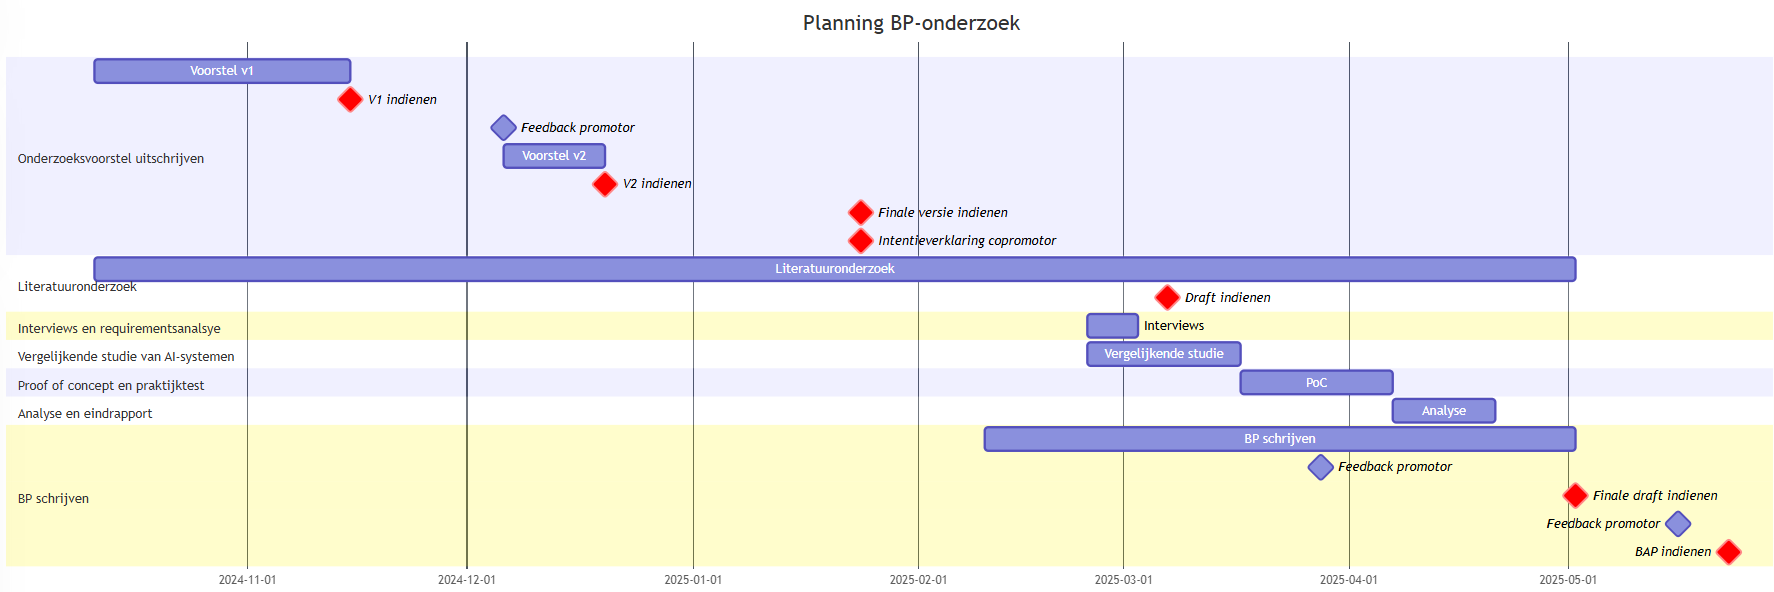
\includegraphics[width=0.5\textwidth]{img/gantt.png}
  \caption{\label{fig:gantt}Gantt planning bachelorproef}
\end{figure}

\begin{figure}[ht]
  \centering
  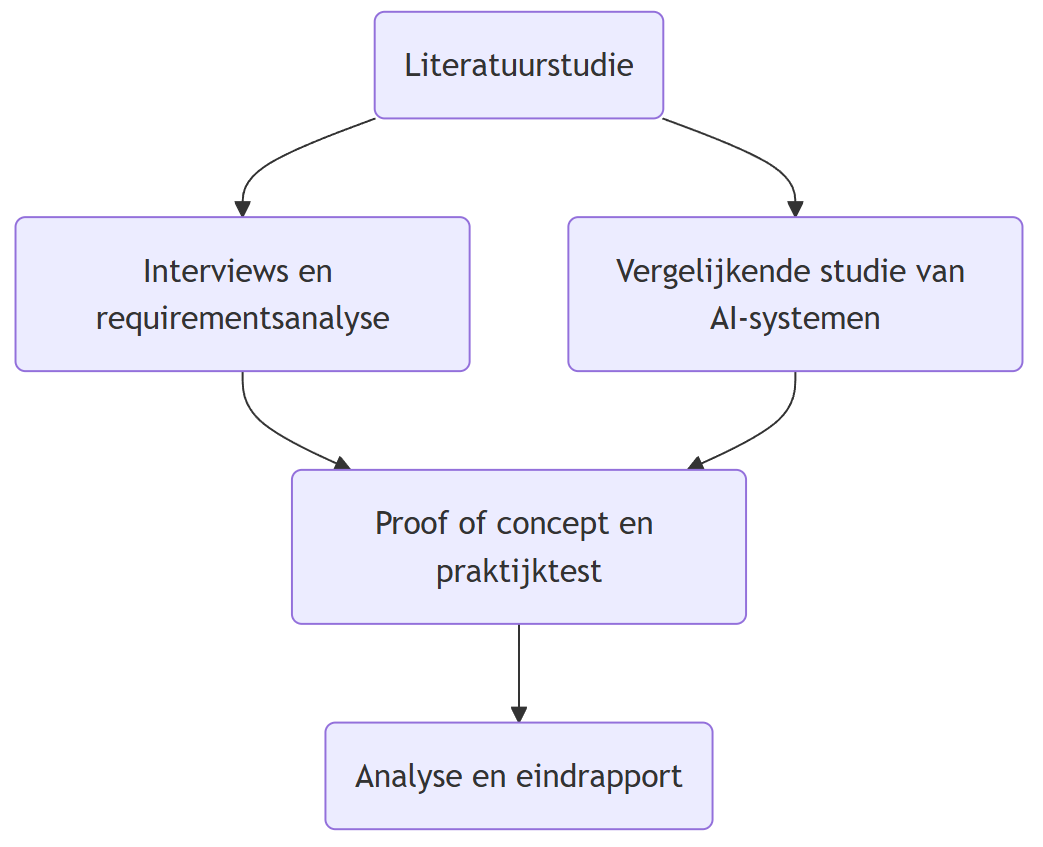
\includegraphics[width=0.3\textwidth]{img/flowchart.png}
  \caption{\label{fig:flowchart}Flowchart bachelorproef}
\end{figure}

%---------- Verwachte resultaten ----------------------------------------------
\section{Verwacht resultaat, conclusie}%
\label{sec:verwachte_resultaten}
Dit onderzoek richt zich op het automatiseren van spelers- en matchstatistieken bij volleybalclub Lindemans Aalst en beoogt een positieve invloed op de nauwkeurigheid en snelheid van dataverzameling, waarmee de club strategisch betere keuzes kan maken. Momenteel worden statistieken tijdens wedstrijden handmatig bijgehouden, terwijl er tijdens trainingen zelfs geen gegevens worden verzameld. Dit handmatige proces is tijdrovend en kan leiden tot inconsistenties in de data. Automatisering biedt potentieel voor een systeem dat in staat is realtime statistieken vast te leggen, zowel tijdens wedstrijden als trainingen, wat resulteert in een meer efficiënte en betrouwbare dataverzameling.

Allereerst wordt een verbetering verwacht in de nauwkeurigheid van gegevensverzameling. Het geautomatiseerde systeem zal naar verwachting 15-25\% nauwkeuriger zijn dan de handmatige methode door het verminderen van menselijke fouten.

Daarnaast wordt een aanzienlijke tijdsbesparing verwacht in de snelheid van data-analyse. Door een AI-gestuurd systeem toe te passen, kan de tijd voor gegevensverwerking en analyse met 30-50\% worden verminderd, wat vooral waardevol is tijdens het dynamische wedstrijdmoment. Het systeem maakt gegevens direct beschikbaar, zodat coaches en spelers tijdens wedstrijden hun beslissingen onmiddellijk kunnen aanpassen aan de realtime prestaties van het team.

Bovendien wordt verwacht dat het systeem de tactische beslissingen en trainingsinzichten van de coaches aanzienlijk zal verbeteren. Met de beschikbaarheid van gedetailleerde statistieken tijdens en na wedstrijden en trainingen zullen coaches in staat zijn om beslissingen te nemen op basis van een hogere kwaliteit en kwantiteit aan data.

De meerwaarde voor Lindemans Aalst ligt in drie hoofdgebieden: betere en snellere besluitvorming, efficiëntieverbetering en langetermijninzicht. Door realtime inzicht te krijgen in prestaties, zowel tijdens wedstrijden als trainingen, kunnen coaches gefundeerde keuzes maken, tijd besparen en diepgaandere analyses uitvoeren. Het systeem voegt waarde toe door historische gegevens op te slaan, waardoor coaches trends en de ontwikkeling van spelers effectief kunnen volgen. De resultaten van dit onderzoek bieden niet alleen een waardevolle tool voor Lindemans Aalst, maar verschaffen ook inzichten die andere sportorganisaties kunnen inspireren om AI-technologieën voor datagedreven analyse en besluitvorming te implementeren.

%%---------- Andere bijlagen --------------------------------------------------
% TODO: Voeg hier eventuele andere bijlagen toe. Bv. als je deze BP voor de
% tweede keer indient, een overzicht van de verbeteringen t.o.v. het origineel.
%\input{...}

%%---------- Backmatter, referentielijst ---------------------------------------

\backmatter{}

\setlength\bibitemsep{2pt} %% Add Some space between the bibliograpy entries
\printbibliography[heading=bibintoc]

\end{document}
